%!TEX root = ../documentation.tex

\chapter{Einsatzbereiche}
Norbert - Your StudyBuddy ist eine Anwendung zum Optimieren des Studienalltags. Doch wie werden die Studierenden darauf aufmerksam?
Ziel ist es dass die Studierenden aus eigener Motivation Norbert benutzen. Dazu muss ein Student in dem jeweiligen Kurs Norbert auf einem Server installieren und einrichten.
Dabei soll die Installation möglichst einfach gestaltet werden.
Vorteil einer Kurs spezifischen Installation ist die Spezialisierung der Software. Es können externe Dienste angegeben werden welche für jeden Kurs unterschiedlich sind. Damit wird z.B. ermöglicht, dass verschiedene Kurse unterschiedliche Mail-Verteiler besitzen können.

\begin{tabularx}{\textwidth}{|l|X|l|l|}
    \toprule
    \textbf{ID-Kürzel} & \textbf{Beschreibung} & \textbf{Prio} & \textbf{Abhängig von}\\
    \midrule
    \endhead
    \hline
    \caption{Einsatzbereiche}
    \label{Einsatzbereiche:tabelle}
    \endfoot
    E-00 & Die Software wird innerhalb eines einzelnen Kurses an der DHBW verwendet. & 1 & \\
    E-10 & Die Software wird zum Verwalten von Dokumenten verwendet. & 2 & \\
    E-20 & Mit Hilfe der Software können Aufgaben geplant werden. & 1 & \\
    E-30 & Die Software wird zum Verteilen von Wissen in Form von Dokumenten oder Aufgaben verwendet. & 1 & \\
    E-40 & Die Software dient zur Aufbereitung wichtiger Informationen aus externen Diensten, wie z.B. einem E-Mail Verteiler oder einer Dropbox. Dadurch können Informationen dieser Dienste in einer einheitlichen Anwendung abgerufen werden. & 2 & \\
\end{tabularx}

%\subsection{Kurssprecher / Freiwillige Studierende}
%Aufmerksamkeit auf die Anwendung kann durch die Partnerunternehmen, die DHBW oder durch die Studierendenvertretung erzeugt werden. Da diese Einrichtungen aber nicht immer schnell und flexibel sind, bietet unsere Softwarelösung die Möglichkeit von einen Studierenden des Kurses selbst gehostet zu werden. Dadurch kann die Software schnell und unabhängig von Unternehmen und staatlichen Einrichtungen verbreitet werden. 

%\subsection{Das duale Partnerunternehmen}
%Die dualen Partnerunternehmen sind meistens die ersten Anlaufstellen der Studierenden. Im Vorpraktikum wird  - soweit möglich - bei Studierenden in höheren Semestern nachgefragt, auf welche Aspekte man in den ersten Semestern den Fokus legen sollte. Doch meistens gestaltet sich dies nicht immer als einfach, denn der Austausch von Dokumenten oder speziellen ToDo's im neuen Semester, haben sich auch die Studierenden der höheren Semester nicht mehr behalten. An diesen Punkten setzt Norbert ein: Das Partnerunternehmen macht auf die Anwendung aufmerksam. Darüber werden zentral alle wichtigen Informationen weitergeben. Zudem könnten die Partnerunternehmen als mögliche Anbieter (Hosting) der Anwendung in Frage kommen und würden somit die Verwaltung der Anwendung übernehmen.
%
%\textit{Warum sollte eine Firma die Anwendung auf eigene Kosten hosten?}
%
%Gerade in den ersten Semestern wird das Lernpensum gerne unterschätzt, Aufgaben vergessen, Termine und Fristen nicht eingehalten. Dies führt häufig dazu, dass bereits nach dem ersten Semester bis zu 50\% der dualen Studierenden ihr Studium abbrechen müssen und das Partnerunternehmen verlassen. Das investierte Geld der Unternehmen und wichtige zukünftige Mitarbeiter sind damit verloren. Durch die Anbietung unserer Softwarelösung besteht die Möglichkeit, dass die Exmatrikulationsquoten verringert werden und mehr dual Studierende ihr Studium erfolgreich bestehen.

%\subsection{Die Duale Hochschule \& Studienvertretung}
%Die Duale Hochschule könnte wie die Partnerunternehmen als Anbieter (Hosting) der Anwendung in Frage kommen. Durch die Vermarktung der Software auf der DHBW-Webseite oder bei Studieninformationstagen kann bereits früh auf die neue Software aufmerksam gemacht werden. Außerdem können über diese Anwendung wichtige DHBW-Pressemitteilungen schnell und kostengünstig verbreitet werden. Nicht zu verachten ist auch, dass die Möglichkeit besteht, dass die Durchfallquoten der DHBW sinken und dadurch mehr Partnerunternehmen, besser Zuschüsse und ein allgemein höheres Ansehen erzeugt werden kann.
%
%Die Studienvertretung kann ähnlich wie die DHBW über die Anwendung über Tagungen, Wahlen, Mitteilungen und Kneipentouren informieren und kommt als potentieller Anbieter in Frage.

\section{Welchen Vorteil bietet Norbert?}
Insbesondere hilft Nobert in folgenden Aspekten:
\begin{enumerate}
	\item Wissensmanagement: Er hilft dem Studenten Aufgaben und Dokumente zu durchsuchen und schlägt ihm aktiv neue Aufgaben oder interessante Dokumente vor.
	\item Wissensweitergabe: Durch die Möglichkeit Aufgaben, Dokumente und Informationen automatisch an Studienkollegen weiterzugeben kann dies den Studenten helfen Ideen für neue Aufgaben zu gewinnen.
	\item Zeitmanagement: Er erinnert den Studenten an eigens definierte Aufgaben oder mögliche Aufgaben.
\end{enumerate}

Die folgende Abbildung verdeutlicht welche Informationen, Termine und Aufgaben der Studierende verpasst haben könnte. 

\begin{landscape}
\vspace*{35mm}
	\begin{figure}[H]
	\centering
	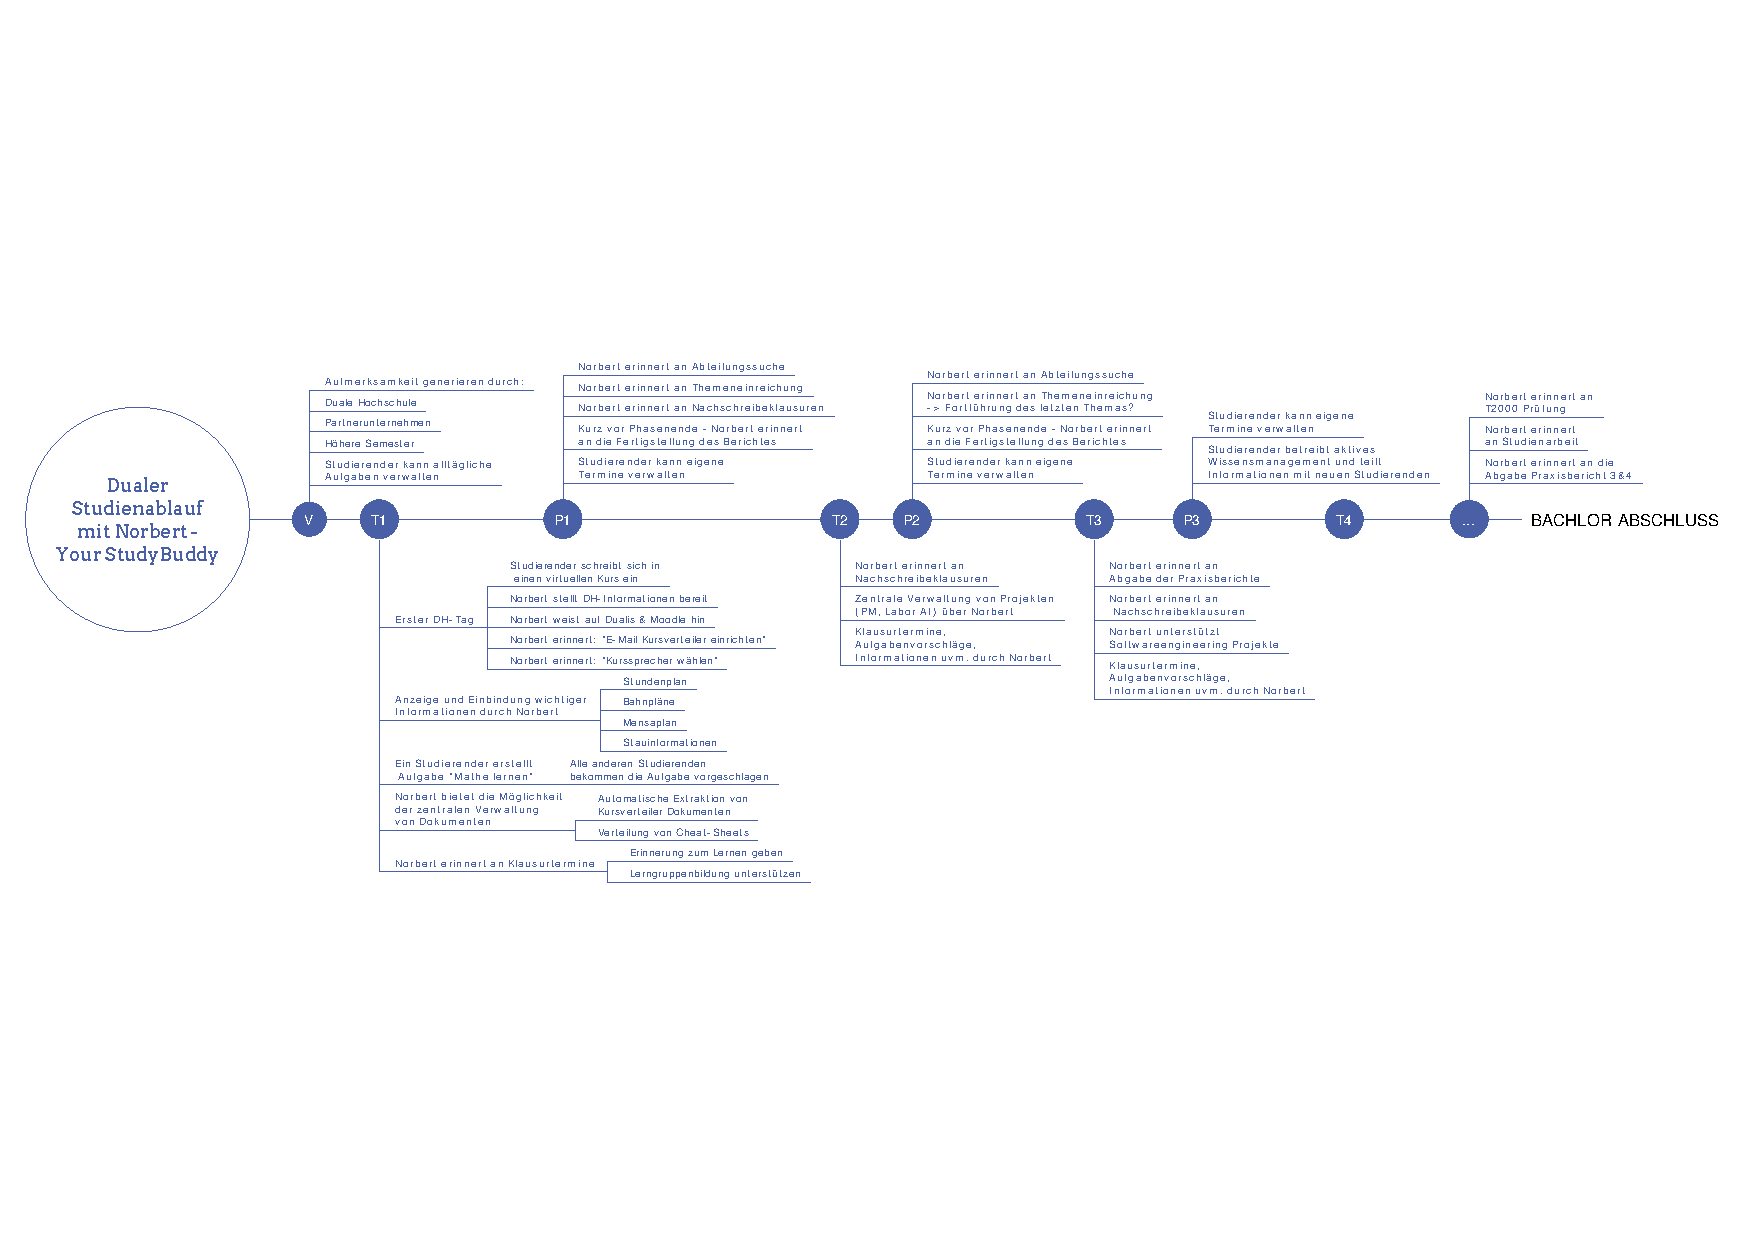
\includegraphics[scale=0.75]{images/timeline.pdf}
	\caption{Lebenslauf eines dualen Studierenden mit Norbert - Your StudyBuddy}
	\end{figure}
	
\end{landscape}
\newpage

\section{Nutzergruppe}

Die Software ist hauptsächlich für Studierende konzipiert - insbesondere für Studierende an der Dualen Hochschule Baden Württemberg. Zum einen gibt es immer Studierende in einem Kurs, die schon bereits kontinuierlich Terminkalender, ToDo-Listen oder Aufgabenmangementtools verwenden. Zum anderen gibt es eine überwiegende Anzahl an Studierenden die dies nur sporadisch und nicht kontinuierlich tun. Durch die Einführung unserer Software in einem Kurs, kann die strukturierte Arbeitsweise der fleißigeren Studierenden von Nutzen für die eher fauleren Studierenden sein. Durch die nützlichen Funktionen von Norbert bietet die Anwendung aber nicht nur den \enquote{fauleren} Studierenden einen Vorteil, sondern die \enquote{fleißigeren} Studierenden müssen nicht mehr viele verschiedene Tools zum Alltagsmanagement verwenden und können ihr gesamtes Studienleben mit Norbert - Your StudyBuddy planen. Da Norbert allen Studierenden eines Kurses automatisch Vorschläge zu Aufgaben, Terminen und Erinnerungen gibt, profitiert der gesamte Kurs von einmalig definierten Einträgen. Weiterhin werden die eher \enquote{faulen} Studierenden dazu angeregt, selbst etwas für das Wohl des Kurses beizutragen und fügen selbst Einträge (Termine, Erinnerungen, Informationen) der Anwendung hinzu. Dadurch kann die Informationssuche und Wissensweitergabe auf den gesamten Kurs übertragen werden und die ist auch für \enquote{fleißigere} Studierende von Vorteil. Selbst wenn nur ein geringer Teil eines Kurses aktiv Informationen und Wissen über Norbert weitergibt, reduziert sich der Gesamtaufwand für alle Studierende drastisch, da der Gesamtaufwand für einen einzelnen Studierenden alleine natürlich viel größer ist.

Weiterhin existieren drei typische Nutzergruppen, die unterschiedliche Funktionalitäten von Norbert unterschiedlich stark verwenden:

\begin{enumerate}
	\item Der \enquote{Informations-Interessierte-Studierende} ist eher an allgemeinen Informationen über die DHBW, den Mensaplan, Bahn Ankunfts- und Abfahrtszeiten, sowie Stauinformationen oder Kurskalenderänderungen interessiert.
	
	\item Der \enquote{Management-Studierende} nutzt Norbert eher zum Planen des Alltags. Er definiert sich feste Aufgaben, Termine und Erinnerungen. Zudem verwendet er die Anwendung um kleinere Projekte innerhalb des Kurses zu verwalten
	
	\item Der \enquote{Informations-Management-Studierende} ist eine \enquote{Mischform} der vorherigen beiden Anwendertypen. Er verwendet alle Funktionalitäten der Anwendung gleichermaßen stark. Dieser Studierende ist stets optimal informiert und hat seinen Studienalltag bestens geplant. 
\end{enumerate}

Ein Ziel von Norbert ist es, dass alle Studierende zu einem Studierenden der letzten Nutzergruppe (3.) werden. Die anderen beiden Anwendertypen (1. \& 2.) können aber als Einstiegspunkt in die Software genutzt werden und als Marketingstrategie um Norbert schneller bekannt zu machen.

%\subsection{Erstsemester-Studierende}
%Ein Erstsemester-Studierender verfügt nur über relativ wenig Wissen, welche Aufgaben und Informationen er zum erfolgreichen Absolvieren des Studiums benötigt. Durch die Vorpraktikumsphase in den Partnerunternehmen werden zwar bereits einige Informationen vorab ausgetauscht, doch oftmals sind diese nicht sehr präzise und geraten schnell in Vergessenheit. Wichtige Termine und Fristen werden zu spät wahrgenommen oder sogar versäumt. Die Vielzahl an Aufgaben in den ersten Semestern überfordern viele Studierende schnell. Zudem fehlen ihm oft die richtigen Informationen zu Beginn des Studiums. Nutzt der Studierende Norbert - Your StudyBuddy bereits zu Beginn des erstem Semesters - oder sogar im Vorpraktikum - bekommt er  das nötige Wissen zum Studium und zur DHBW mitgeteilt. Weiterhin bekommt er sinnvolle Aufgaben und Termine aus vorherigen Jahrgängen vorgeschlagen und kann sich an ToDo's der Studienkollegen orientieren. Somit findet eine Wissensweitergabe statt. Durch dieses optimierte Wissens- und Aufgabenmanagement, welche speziell auf duale Studierende abgestimmt ist, hat der Studierende mehr Freizeit, die er für Hobbys, Kneipentouren und Partys nutzen kann.
%
%\subsection{Erfahrene Studierende}
%Studierende in den höheren Semestern nutzen die Anwendung nicht mehr hauptsächlich, um einfach nur Informationen zu erhalten, sondern können über die Anwendung Aufgaben und Projekte verwalten. Außerdem geben sie Wissen an Erstsemester-Studierenden weiter. Somit profitieren die neuen Studierenden von den Erfahrungen  der vorherigen Semestern. Dabei geht die Wissensweitergabe automatisiert vonstatten, sodass niemand zusätzlich Termine und Aufgaben für andere Studierende erstellen muss. Die Integration von verschiedenen häufig genutzten Diensten ermöglicht Informationen in einer Anwendung zu bündeln und auf einen Blick darzustellen. Durch einen optimierten und strukturierten Studienalltag hat der erfahrene Studierende mehr Zeit zum Bearbeiten von Projekten, Studienarbeiten und kann sich besser auf Prüfungen vorbereiten.
